%!TEX root = ../ap_gcc.tex

\section{Unix fact extraction mechanism in detail}

In this section we want to explain the unix fact extraction mechanism in more detail. Especially we want to explain how we implemented the callmon library, the executable patching mechanism and metacreator.

\subsection{Overview}

First of all we want to give a quick overview about the whole workflow of the fact extraction tool chain. These are the steps if you want to instrument your application and visualize the trace in CGA:

\begin{enumerate}
	\item Building the application with special compiler flags and linking the callmon.{dll,dylib,so}.
	\item Patching the executable results in an executable with just NOPs and a patch file (patch clean).
	\item Patching the executable with the help of an include/exclude file so that we just have specific logging enabled (patch).
	\item Executing the application.
	\item Start logging with the cga toolbar creates a pre modinfo file.
	\item During the logging callmon writes cmlog files for every thread.
	\item Stop logging with the cga toolbar creates a post modinfo file.
	\item The metacreator takes the cmlog and modinfo files and creates a .callmon file
	\item Import and visualize the trace with CGA.
\end{enumerate}

The unix fact extraction mechanism is a non-intrusive, light-weight way for logging function calls in C/C++ software systems that are built with GCC version 4.2 or higher. Callmon is used to log the sequence of function calls from a running application. Time stamps are obtained for both entry and exit points of each function. The logging mechanism does not slow down the users application when being deactivated. This is obtained by patching the executable and libraries files of the application. All assembler instructions, which are needed for logging are replaced by assembler NOPs. If the user wants to log certain activities he can patch the executable again so that the logging for this functions are now active. For more detailed information about the process have a look at the tutorial section \ref{sec:Tutorial}.

\subsection{Callmon}

The central element of the tracing mechanism is callmon. Callmon is a static library, which you have to link against the application you want to instrument. But the most important part is the GCC parameter -finstrument-functions. We will explain this later in more detail. To get an overview about the classes which are involved in the tracing mechanism have a look at figure \ref{fig:unixfe_figure1}.

\begin{figure}[ht]
\centering
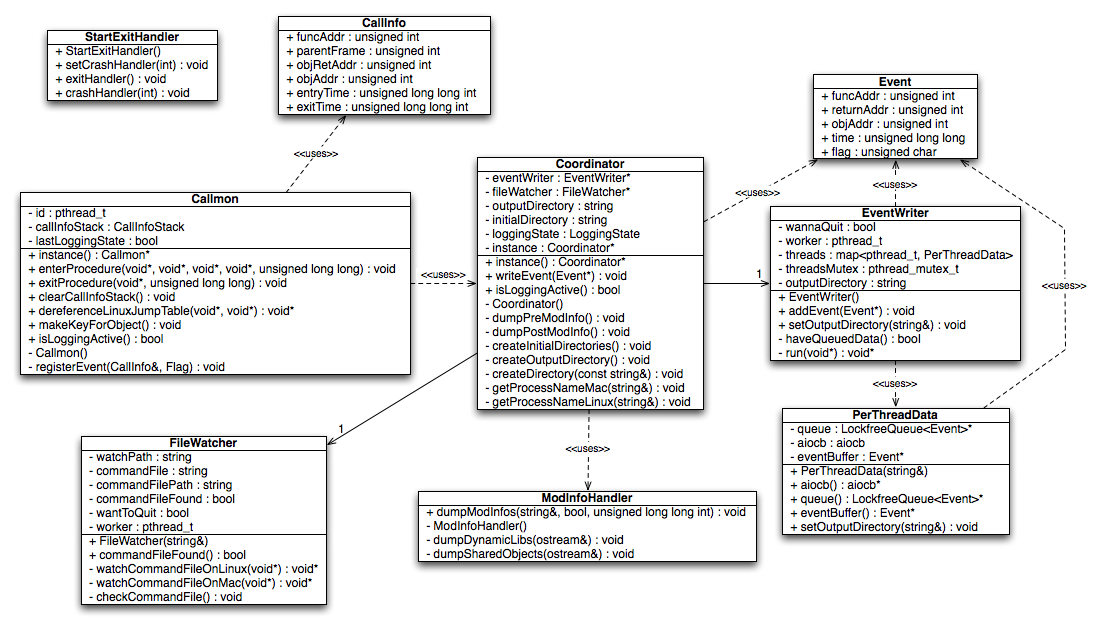
\includegraphics[width=16cm]{images/callmon_class_diagram}
\caption{Class diagram of the callmon library}\label{fig:unixfe_figure1}
\end{figure}

The \verb=StartExitHandler= \todo{new font here? use it all over?} helps to set up crash handlers for the most common signals (SIGINT, SIGILL, SIGSEGV, SIGFPE, SIGTERM, SIGABRT, SIGBUS, SIGHUP)\footnote{\url{http://en.wikipedia.org/wiki/Signal_(computing)}} and an exit handler right after startup (before main). We ensure that the constructor of the \verb=StartExitHandler= is executed before the main routine of the application with the help of a static variable. Static variables are initialized before the first call of the applications main routine. The \verb=exithandler()= function deletes the \verb=Coordinator= instance. If the application crashes the crash handler gets executed, which processes just a normal shutdown and cleanup.

\verb=Callmon= provides the functionality to log function enters and exists. Every thread of the application has its own \verb=Callmon= object. The \verb=Coordinator= is responsible to create the \verb=EventWriter=, the \verb=FileWatcher= and the directory structure for the log files. It also coordinates if callmon is allowed to log an event. The \verb=EventWriter= runs in its own thread and receives events from all the applications threads through a lock free queue. It uses asynchronous I/O to fill the thread specific log files. The \verb=FileWatcher= runs also in its own thread and listens on events of the file system. If a file called callmond.cmd is created or deleted we indicate this with a boolean. The \verb=ModInfoHandler= is responsible to write at the beginning and the end of the logging a list of used libraries and their start address to a modinfo file. Some classes are explained in more detail in the next sections.

As mentioned more early, one of the key elements is the GCC parameter -finstrument-functions. With this option GCC inserts calls to \verb= __cyg_profile_func_enter()= and \verb=__cyg_profile_func_exit()=. When an instrumented function is called, \verb= __cyg_profile_func_enter()= is also called, passing in the address of the function called as \verb=funcAddress= and the address from which the function was called as \verb=callSite=. When a function exits, the \verb=__cyg_profile_func_exit()= function is called, passing the function's address as \verb=funcAddress= and the actual site from which the function exits as \verb=callSite=.

We implemented both functions (see callmon.cpp), which collect the following data if logging is active:
\begin{itemize}
	\item Function address
	\item Call site
	\item Frame pointer
	\item Parent frame pointer
	\item Object pointer (this pointer)
	\item Entry and exit time
\end{itemize}

On Linux when a function of a shared library gets called from the main executable, \verb=__cyg_profile_func_enter()= reports the wrong function address. It just tells the address in the jump table, not where the real function code is located. Therefore we have to correct the function address with the help of \verb=dereferenceLinuxJumpTable()=, which walks over the jump table and finds the real address.

\begin{figure}[ht]
\centering
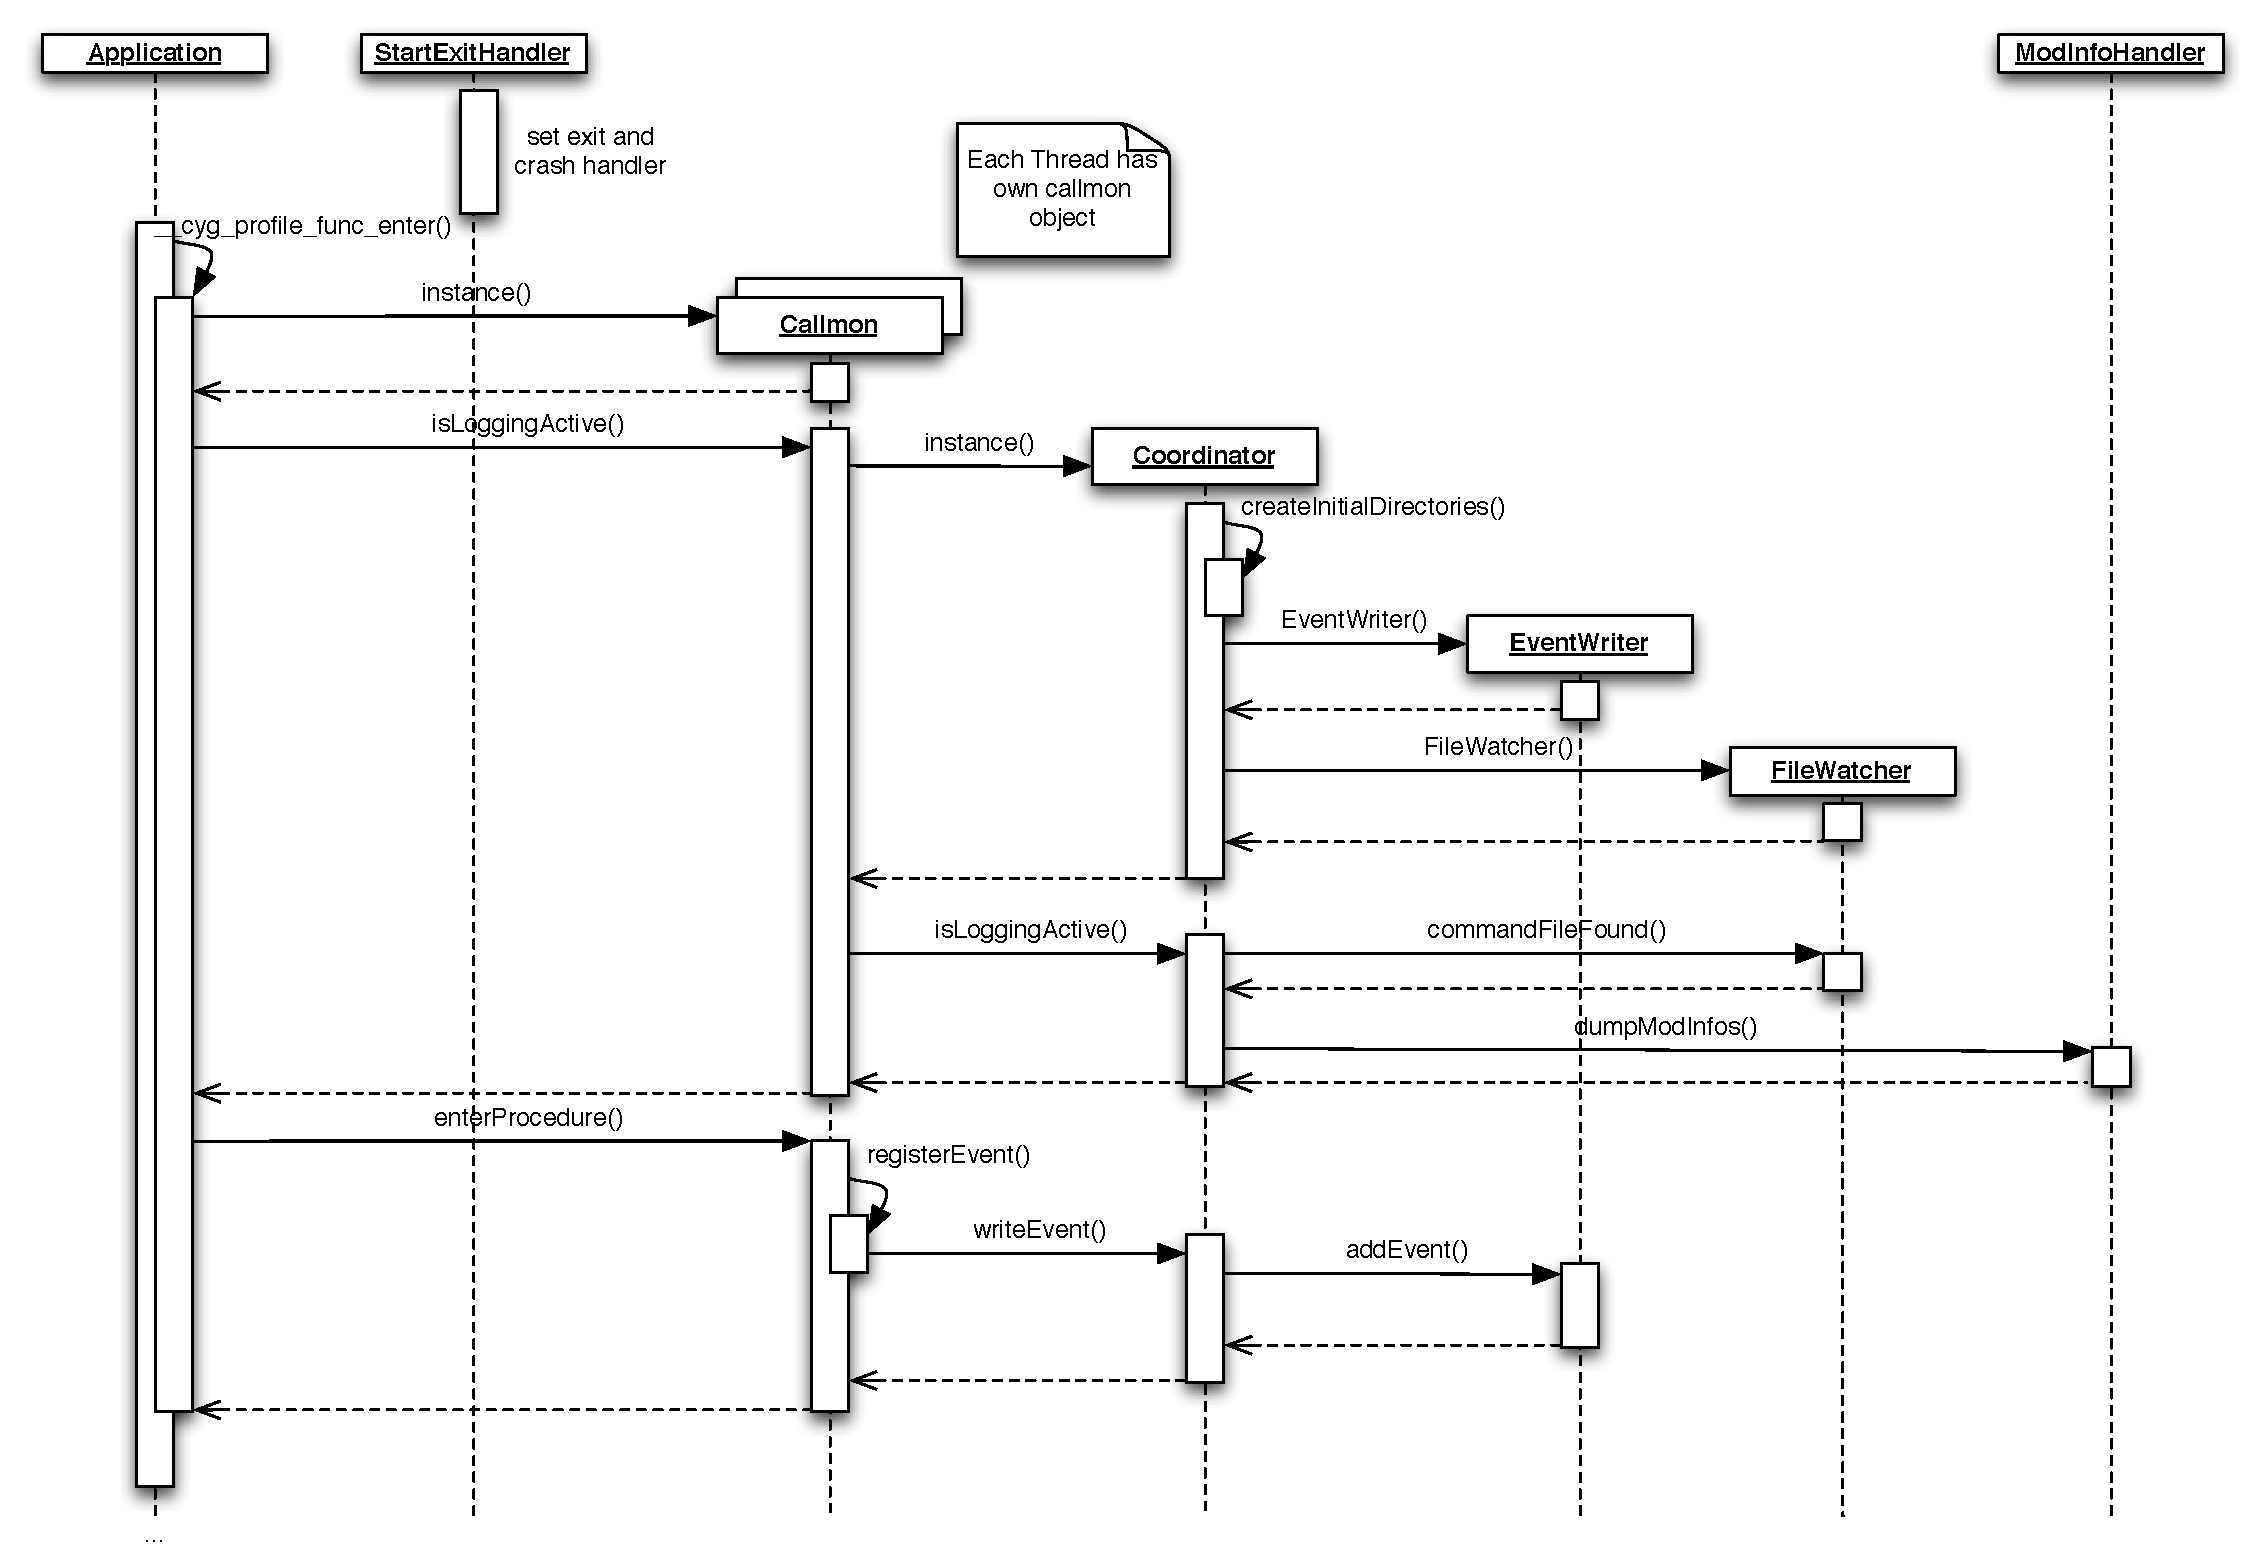
\includegraphics[width=16cm]{images/callmon_sequence_diagram}
\caption{Sequence diagram of the function enter process}\label{fig:unixfe_figure2}
\end{figure}

Figure \ref{fig:unixfe_figure2} illustrates a simplified event logging process for the first \verb=__cyg_profile_func_enter()= in which we assume that logging is enabled. If the user starts the application the constructor of the \verb=StartExitHandler= is executed up front and the exit and crash handler is set up. In the next step the \verb=__cyg_profile_func_enter()= is called. On Mac OS X and Linux exists no DllMain mechanism, so we have to use lazy initialization and thread-local storage to address this problem. A callmon instance is requested and created on demand if there is no instance for this thread. The pointer to the callmon instance is stored in the thread-local storage. After the lazy	initialization of the callmon object we check if logging is active. To determine if we are allowed to log an event, we need to create a coordinator (singleton), which is also responsible to initialize the event writer and file watcher (detailed information can be found in the following sections). Both the event writer and file watcher run in their own thread. After this, callmon can ask the coordinator if logging is active or not. The whole logging mechanism is enabled if the file watcher finds a \verb=callom.cmd= file in the callmon home directory. If this was the start of a new logging procedure we also write a pre modinfo file to the specified output directory.

In the next step \verb=__cyg_profile_func_enter()= collects the whole data we need to write an event to the thread specific log file. This data is passed to the \verb=enterProcedure()= of the callmon instance. In this function we push a new \verb=CallInfo= object on our shadow stack. On the one hand we need the shadow stack to recognize if there was an exception during the execution, because then we will have a different return behavior of the function. On the other hand the shadow stack is needed to address the problem if we have an unprofiled function call between two profiled functions. Then we call the \verb=registerEvent()= function, which creates a new \verb=Event= object. The Event is then written with the help of the \verb=EventWriter= to a log file.

The whole procedure for \verb=__cyg_profile_func_exit()= is very similar, beside that the \verb=exitProcedure()= pops the shadow stack until we find a call record that matches the current stack layout. If we did not find a call record that matches we register an exceptional event.

The structure of the event which is also written to the cmlog files looks like the following:
\begin{itemize}
	\item Function address
	\item Return address
	\item Object address
	\item Entry or exit time
	\item Flag (entry, exit or exception)
\end{itemize}

\subsubsection{Coordinator}

The \verb=Coordinator= class uses the singleton design pattern so that we just have one \verb=Coordinator= instance at a time. One of the important tasks of the class is to set up the initial directory structure where callmon stores the log and mod info files. Therefore the function \verb=createInitialDirectories()= is called in the constructor, which creates the following directory structure:

\begin{verbatim}
  CALLMON_HOME or current working directory /logs/<appname>/
\end{verbatim}

On Mac OS X the name of the currently running application ($<$appname$>$) is determined with the help of the \verb=kinfo_proc= structure. On linux we use the process file system, which is a pseudo file system used to access process information from the kernel. We get the name of the application by resolving 

\begin{verbatim}
  /proc/<pid>/exe (symbolic link)
\end{verbatim}

Another important task of the \verb=Coordinator= is to create the \verb=EventWriter= and \verb=FileWatcher=, which will be explained later in more detail. But the most important functionality of the \verb=Coordinator= is to indicate if callmon is allowed to log the function enters and exits in a lockfree way, even in multithreaded environments. This is accomplished by using atomic operations. Since version 4.2 GCC provides a function called \verb=__sync_bool_compare_and_swap()=, which sets and test a variable in an atomic way. The \verb=Coordinator= instance asks the \verb=FileWatcher= if logging is active or not. If logging is active we have to check if we are at the beginning of a new logging cycle. At the beginning of a logging cycle we have to set up certain things such as creating the output directory for the log files, write a pre modinfo file and set the output directory of the \verb=FileWatcher=. The output directory for the current trace is:

\begin{verbatim}
  CALLMON_HOME or current working directory /logs/<appname>/<date_time>
\end{verbatim}

If we are not allowed to log we have to check if we are at the end of a logging cycle. At the end of a logging cycle we write a post modinfo file to the current output directory.

\subsubsection{Modinfo handler}

The \verb=ModInfoHandler= provides the functionality to write a pre modinfo file at the beginning of a new trace and a post modinfo file at the end of the trace. The first line of the modinfo file is the \verb=queryPerformanceFrequency=, which is not used anymore. To be consistent with the Windows callmon implementation we still write this as the first line in the modinfo file. The central element of the modinfo file is the list of libraries and their start addresses the application is using. The format of the file looks like this:

\begin{verbatim}
  queryPerformanceFrequency: 1
  00000000 /path/to/lib
  ...
\end{verbatim}

To get the start address and the path of the libraries on Mac OS X we use the following functions the linker provides. The function \verb=_dyld_image_count()= returns the current number of images mapped in by the dynamic linker. The start address can be resolved with the help of \verb=_dyld_get_image_vmaddr_slide(image_index)= and to get the name of the library we use \verb=_dyld_get_image_name(image_index)=, which returns the name of the image.

On Linux the \verb=dl_iterate_phdr()= function walks through the list of an application's shared objects and calls the function callback once for each object. The first of the three parameters the callback gets, is a pointer to a \verb=dl_phdr_info= structure, which contains the start address and the name of the shared object.

With the help of the pre and post modinfo files the metacreator knows which symbols it has to extract. Moreover that the metacreator obtains the corresponding address offsets for the extracted symbols from the pre and post modinfo files.

\subsubsection{Filesystem events}

The \verb=CGA Toolbar= is a simple QT application which simplifies the whole logging process. Besides some small fixes for cross platform compatibility it is exactly the same application as the previous Windows version. With the toolbar the user can start and stop the logging mechanism and start the metacreator for traces of a specific application. The interesting part of the toolbar is in order to start and stop the logging mechanism, it creates an empty file called \verb=callmon.cmd= at the path specified by the \verb=CALLMON_HOME= environment variable. To stop logging the toolbar removes the \verb=callmon.cmd= file.

That is the reason why we need to listen on filesystem events to start and stop logging. In both cases we listen for changes on a specific path and set a variable to true if we find the \verb=callmon.cmd= file or to false if not.

On Mac OS X we use the kernel event notification mechanism \verb=kqueue= and \verb=kevent=. The \verb=kqueue()= system call provides a generic method of notifying the user when an kernel event happens or a condition holds, based on the results of small pieces of kernel code termed filters. The \verb=kevent()= system call is used to register events with the queue, and return any pending events to the user. The only downside of this solution is that we do not get the exact change as an event, we just get the event that a file was created or deleted at the specified path. So we have to check manually with \verb=open(file)= if the file exists. The \verb=kevent()= system call is blocking for a specified timeout or until there is a pending event. In our case we specified a timeout of one second, so that we can interrupt the loop if we want to suspend the \verb=FileWatcher= thread.

The Linux way uses \verb=inotify= which is a Linux kernel subsystem that provides file system event notification. The \verb=inotify_init()= call creates a new instance and returns a file descriptor which all events are read from. With the help of \verb=inotify_add_watch()= we add a new watch for the specified path. We can now call \verb=read= on the file descriptor. This call will block until we get an event. The \verb=inotify_event= structure provides us with enough information so that we can check if the \verb=callmon.cmd= file was created or deleted.

\subsubsection{Event writer} 

event writer (own thread), PerThreadData, setOutputdirectory, Mutex

The lockfree queue is thread safe as long as there is only one reader and one writer. It has a static size which has to be provided at initialization. \todo{TODO: explain in more detail}

\subsubsection{Asynchronous I/O}

We use asynchronous I/O to write the logged function entries and exits to a thread specific log file. The \verb=EventWriter= runs in its own thread and stores the received events, as described in the previous section, in a lockfree queue. If the \verb=EventWriter= thread is scheduled we check if there are any events in the queue and write them to the log file. A very simple approach to write the events to the log file would be synchronous I/O, which blocks the progress of a program until the operations are completed. The alternative is to start the communication and then perform processing that does not require that the I/O has completed. This is called asynchronous I/O and is much more efficient then synchronous I/O.

To perform asynchronous I/O we use the POSIX standard for asynchronous input and output. \verb=aio_write()= gets as parameter a \verb=aiocb= structure which stores a file descriptor, file offset, the location of the buffer we want to write and the length of transfer. For more specific information have a look at the \verb=aio= man page.

\subsection{Patch and Patchclean}

Unfortunately the original patch and patchclean tools had some implementation specific limitations which made a direct port to UNIX hardly feasible.

\todo{Reasons: Windows API, PE code, DIA API, nur enter}

Also the requirements on Linux and Mac OS X where different because of the fact that GCC always compiles the exit instrumentation into the functions and enforces its call on all ways out of a function.

Because of the above mentioned reasons we decided to re-implement the patching tool chain for Linux and Mac OS X.  This 2 new UNIX patching tools reside in the \emph{factextraction/unix/unixfactextraction/} directory.

\todo{Explain architecture, similar to windows, patch files (qdatastream), }


\subsubsection{ELF patching} 

file specifics, offsets, objdump, see requirements


\subsubsection{Mach-O patching}




\subsection{Metacreator} 

\subsubsection{Line number caching} 
